\documentclass{sig-alternate-2013}
\usepackage[latin1]{inputenc}
\usepackage{url}
\usepackage{listings}
\newfont{\mycrnotice}{ptmr8t at 7pt}
\newfont{\myconfname}{ptmri8t at 7pt}
\let\crnotice\mycrnotice%
\let\confname\myconfname%

\permission{Permission to make digital or hard copies of part or all of this work for personal or classroom use is granted without fee provided that copies are not made or distributed for profit or commercial advantage, and that copies bear this notice and the full citation on the first page. Copyrights for third-party components of this work must be honored. For all other uses, contact the owner/author(s). Copyright is held by the author/owner(s).}
\conferenceinfo{GECCO'14,}{July 12--16, 2014, Vancouver, BC, Canada.}
\copyrightetc{ACM \the\acmcopyr}
\crdata{978-1-4503-1964-5/14/07. \\
Include the http://DOI string/url which is specific for your submission and included in the ACM rightsreview confirmation email upon completing your ACM form}

\clubpenalty=10000
\widowpenalty = 10000
\begin{document}
%
% --- Author Metadata here ---
\conferenceinfo{GECCO'14} {Vancouver, Canada}
\title{Assessing different architectures for evolutionary algorithms in JavaScript}
\subtitle{}
\numberofauthors{6}
\author{
\alignauthor
J.J. Merelo, Pedro Castillo, M.G. Arenas, Antonio Mora\\
       \affaddr{University of Granada}\\
       \affaddr{GeNeura, ETSIIT + CITIC}\\
       \email{jmerelo,pedro,\\mgarenas,amorag@geneura.ugr.es}
\alignauthor
Anna I. Esparcia-Alc�zar\\
\affaddr{S2 Grupo}\\
\email{aesparcia@s2grupo.es}
\alignauthor
V�ctor Rivas-Santos\\
\affaddr{Universidad de Ja�n}\\
\email{vrivas@ujaen.es}
}

\maketitle
\begin{abstract}
After more than fifteen years, JavaScript has finally risen as a popular
language for implementing all kind of applications, from server-based
to rich Internet Applications. The fact that it is implemented in the browser and in server-side tools makes it interesting for
designing evolutionary algorithm frameworks 
that encompass both
tiers, but besides, they allow a change in paradigm that goes beyond
the canonical evolutionary algorithm. 
In this paper we will experiment
with different architectures, client-server and peer to peer to assess which ones offer most advantages in terms of
performance, scalability and ease of use 
for the computer scientist. All implementations  have been released as open source, and besides showing that the concept of working with evolutionary algorithms in JavaScript can be done efficiently, we prove that a master-slave parallel architecture offers the best combination of time and algorithmic improvements in a parallel evolutionary algorithm that leverages JavaScript implementation features.

\end{abstract}

% A category with the (minimum) three required fields
\category{H.4}{Information Systems Applications}{Miscellaneous}
%A category including the fourth, optional field follows...
\category{D.2.8}{Software Engineering}{Metrics}[complexity measures, performance measures]

\keywords{Javascript, node.js, parallel evolutionary algorithms, asynchronous evolution}

\section{Introduction}

JavaScript (JS from now on) is an embedded language, interpreted by internet browsers,
that uses classes and objects, uses functions as first-rate types and
is dynamic and weakly typed-checked. These features make
it an ideal language for quick prototyping and productive
programming. Due to Google's introduction of the V8 command-line
interpreter and its adoption by  {\tt node.js}, Javascript is one of the most popular development languages, and the only one of
which it can be said that it is truly ubiquitous.

What we propose in this paper is to measure different ways of
implementing distributed evolutionary algorithms using JS. It
has already been proved that implementation matters because every language offers new ways of
implementing evolutionary algorithms. 

\section{An evolutionary algorithm in {\tt node.js}}
\label{sec:node}
An open source library, which is introduced in this paper, for evolutionary algorithms running under{\tt node.js} (which, from now on, we will simply call Node)  has been released. It has been intended mainly as a proof of concept, including
the bare minimum to run an evolutionary algorithm: a single mutation
and crossover operators, tournament selection and a few test
functions, including the Trap function that has been selected for
making the experiments in this paper:
$$
  T(x) = \left\{ \begin{array}{rl} 
      a*(z-x)/z &\mbox{ if  $x<= z$} \\
    b*(x-z)/(l-z) &\mbox{ if  $x>z$} \\
\end{array}\right.
$$
where $x$ is the number of ones in the block, $l$ is the length of the
block, $z=3$, and $a=1$ and $b=2$. Experiments have been carried out with blocks of length equal to 30, 40 and 50. With respect to number of individual, it was found that 512, 1024 and 2048 are the right size to find the solution to the 4-trap problem of sizes 30, 40
and 50, respectively.

Node is a JS interpreter based on the V8 virtual machine created by Google. It is
designed to deal with asynchronous input/output by default, also including an event model that makes event-driven programming extremely easy.

From the point of view of parallel evolutionary algorithms, instead of
the classical evolutionary sequential loop, a long-lasting loop must be done this way in
Node:
\begin{lstlisting}
generate_population();
do_evolution();

function do_evolution(){
  single_generation();
  if (time_to_migrate()) {
    migrate_out();
    migrate_in();
  }
  if ( !evolution_end() ) {
    do_after_callbacks( do_evolution());
  }
}
\end{lstlisting}






The results of the experiments to size the population are shown in
Figure \ref{fig:pop}, which shows that 512, 1024 and 2048 are the
right size to find the solution to the 4-trap problem of sizes 30, 40
and 50. 

\section{Testing distributed evolutionary architectures}
\label{sec:dist}
The easiest way of creating a distributed application using Node is
adding a RESTful interface to it using {\tt express.js}; in fact,
RESTful interfaces are quite efficient and have been tested already in
distributed EC experiment	,
finding that they add a small overhead to communications and, besides,
can be accessed from a variety of languages, from {\tt node.js} itself to
JQuery (a JavaScript library) in the browser. This gives us room for
growth, but for the time being we are interested only in showing that
a few lines of code can be used to convert a single-process
evolutionary algorithm into a distributed evolutionary one.

We will test two different regimes:\begin{itemize}
\item {\em P2P}: in it, every {\em node} (or process) communicates with the
  rest.
\item {\em pool-based} communication of one client with other is only
  done through the server, with each program acting independently and
  knowing only about this server. 
\end{itemize}

These two implementations will be described in detail in the next two
sections, after which we will present and compare the result of the experiments
using them.

\subsection{Experiments and results}

We tested if the approach is valid and if by dividing the
population in several processes we obtain any kind of improvement. The
machine is the same as above and except for some errors all
experiments have been repeated 30 times to achieve statistical
significance. The point of the
experiment is, anyways, to see how the division of the population
influences the performance. 


What we can conclude from this set of experiments is that a single
machine is able to support a good amount of processes running in
parallel, and that adding at least one process can increase speed
significantly without too much effort (a few lines of code) from the  programming point of view. 

However, this programming effort can be used in a different direction,
and that is what we have attempted with the pool architecture,
% Antonio - he puesto aqu� pool architecture en lugar de other architecture
 with
clients all working against a single server. 

%
\begin{figure}[htb]
\centering
   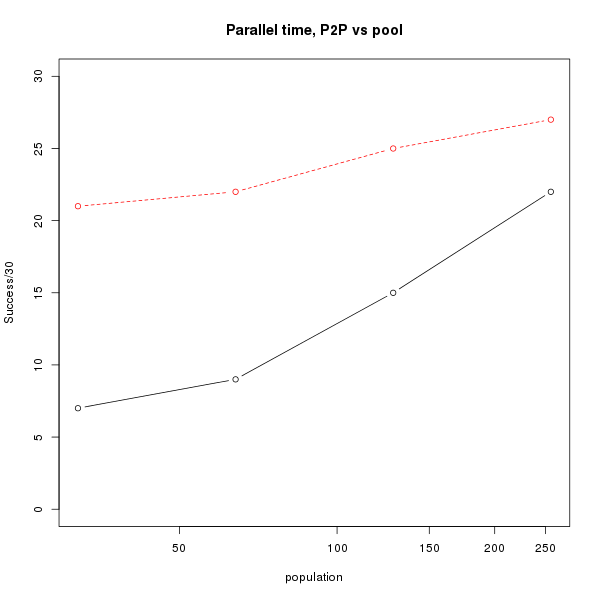
\includegraphics[scale=0.4]{par-pool-hits-pop.png}
\caption{Number of successful runs out of 30. Black, solid line
  corresponds to the P2P architecture, light-colored, dashed
corresponds to the single-server architecture (pool).}
\label{fig:p:hits}
\end{figure}
% Antonio - he puesto aqu� 'pool' porque las im�genes pueden salir lejos una de otra y as� son autocontenidas.


From the point of view of the operating system load, no
great change is observed with the addition of one process ($n$ client
processes + server) to the pool. But a more dramatic change of scenario is shown in Figure
\ref{fig:p:hits}, which shows that the success rate increases
drastically.

This conclusion is reached on top of the fact that JavaScript, its
implementation in {\tt node.js}, and the simple library we are presenting in
this paper, are valid platforms for performing distributed computation
experiments, since they allow to create rapid prototypes to
concentrate on system architecture and the solution of problems via
evolutionary algorithms. 


\section{Conclusions}

In this paper we set to prove the worth of a {\tt node.js}-based distributed
evolutionary algorithm. {\tt node.js} is a emerging platform which is
receiving a lot of interest in the open source and enterprise arena,
but not so much in the scientific community so our intention was to
introduce it to the evolutionary computation (EC) community by proving its
value as a platform for EC experiments. A basic EC library has been
created and released, so it is available to the researches. The
library can be expanded and, being open source, can be adapted and
suited to the needs of any particular user; due to the expansion of
the JavaScript and {\tt node.js} community, it should be increasingly easy
to find people interested and skilled enough to work in evolutionary
algorithms using JavaScript and {\tt node.js}, and, from the other end, it could get
the {\tt node.js} community interested in our area, which might prove the
source of interesting problems that can be dealt with from the point
of view of metaheuristics.




%ACKNOWLEDGMENTS are optionalndn
\section{Acknowledgments}
This work has been developed thanks to the funds provided by local
CEI-BioTIC grant  CANUBE (CEI2013-P-14) and national ANYSELF project (TIN2011-28627-C04-02). 


%
% The following two commands are all you need in the
% initial runs of your .tex file to
% produce the bibliography for the citations in your paper.
\bibliographystyle{abbrv}
\bibliography{geneura,javascript,ror-js}  % sigproc.bib is the name of the Bibliography in this case

\end{document}
